\documentclass{article}
\usepackage[pdftex]{graphicx}
\usepackage[margin=1in]{geometry}
\setlength{\parindent}{0mm}
\newcommand{\tab}{\hspace*{2em}}
\begin{document}

\begin{center}
{\LARGE\textbf{CARLOS ANDRES CAICEDO ARELLANO}}\\
\end{center}

\begin{center}
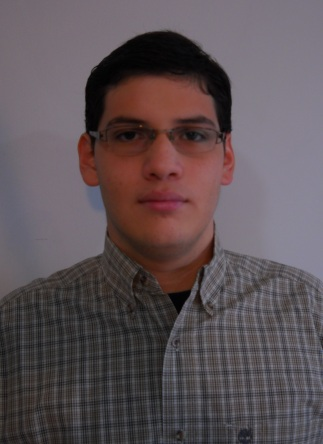
\includegraphics{myimage.png}\\
\end{center}

{\large\textbf{Datos Personales:}}\\

\textbf{Estado Civil:} Soltero

\textbf{Cedula de Identidad:} 093110038-2

\textbf{Lugar y Fecha de Nacimiento:} Guayaquil, Mayo 26, 1993

\textbf{Telefonos:} (T) 2852549 – (C) 093793038

\textbf{Ciudad:} Guayaquil

\textbf{Correo Electronico:} carloscaicedo2002@hotmail.com

\textbf{Direccion Domiciliaria:} Santa Cecilia, Cond. Panorámico Mz. Z, Dept. 8, Peatonal 2da entre la 7ma y la 9na.\\

{\large\textbf{Estudios Realizados:}}\\

\textbf{Primaros:} Liceo Bilingue Vida Nueva (1997-2005)

\textbf{Secundarios:} Colegio Politecnico (COPOL) (2005-2011)

	\tab{\tab{Bachiller en Ciencias}}

	\tab{\tab{Especializacion: Ingenieria (Fisico Matematico)}}

\textbf{Universitario:} Escuela Superior del Litoral (ESPOL) (2011-en la actualidad)

	\tab{\tab{Cursando 2do Año, en la Carrera de Ingenieria en Computacion}}\\

{\large\textbf{Idiomas}}\\

\textbf{Ingles:} 100% hablado y escrito 

	\tab{\tab{Finalizacion del curso de ingles del COPOL con los mas altos honores (2011)}}

\textbf{Frances:} 10% hablado y escrito\\
 
\newpage

{\large\textbf{Certificados Obtenidos}}\\

\begin{itemize}
\item{TOEFL (Internet-based Test) – 109}

\item{SAT: 630 Reading; 740 Math; 670 Writing}

\item{SAT Subject Tests: 730 Mathematics Level 2; 650 Physics; 800 Spanish with Listening}

\item{Microsoft Certified Application Specialist en Microsoft Word, Microsoft Excel y Microsoft PowerPoint (2008-2010)}

\item{Internet and Computing Core Certification (Computer Fundamentals, Key Applications y Living Online) (2007)}

\item{Certificado del Bachillerato Internacional:}
 
\begin{itemize}
	\item{Matematicas NM 5}

	\item{History NM 4}

	\item{Language B Ingles NS 7}
\end{itemize}

\item{Suficiencia de Ingles CELEX, Escuela Superior Politécnica del Litoral.}\\
\end{itemize}

{\large\textbf{Cursos Realizados}}\\

\begin{itemize}
\item{Nivel Advance 10 del COPOL English Institute, Febrero 2011-Abril 2011}
\item{CELEX Nivel 1 de Francés, Febrero-Abril 2010}\\
\end{itemize}

{\large\textbf{Referencias Personales}}\\

Tec. Monica Franco

Catedratica – Coordinadora Proyecto Periodismo CAS

Colegio Politecnico

(T) 2991186 – (C) 097200681 \\

Lic. Carlos Villafuerte

Editor Noticias - 24 Horas

Teleamazonas

(T) 2273964 – (C) 098145101

\end{document}